\documentclass[11pt]{article}
\usepackage{icmlko}
\begin{document}

\title{무게를 고치려다 못 고쳤다 --- 그리고 판이 새 도메인을 못 맞힌다는 것을 알았다}
\author{월드모델 실험실}
\date{노트 380 · 2026년 8월 1일}
\maketitle

\begin{abstract}
노트 379가 펀딩 449건을 유보에 넣자 판이 $0.4620 \to 0.4057$ 로 내려갔는데
\textbf{그중 86\%가 펀딩의 무게가 80에서 529로 커진 몫}이었다. 무게가
채점된 유보 행 수라 \emph{많이 긁으면 발언권이 커진다.} 고치려 했다.

\textbf{첫 수치는 솔깃했다.} 저장된 관문 열 팔을 무게 규칙 넷으로 다시
판정하니 균등 무게가 신호대잡음(\,$|$차$|\div$짝SD\,)을 $0.42 \to 0.64$ 로
\textbf{52\% 올리고}, 배포에 떠넘기는 판정이 7건에서 3건으로 줄고,
방향이 뒤집히는 팔은 없었다. 게다가 균등은 판을 $0.4057 \to 0.3767$ 로
\emph{내리므로} 점수 욕심으로 고르는 것도 아니었다.

\textbf{갈랐더니 두 번 무너졌다.} 첫째, 그 이득은 팝업 팔에 몰려 있다 ---
팝업 실험 여덟에서 $0.45\to0.68$ 인데 팝업 아닌 두 팔은 표본이 너무 얇고
그중 하나는 진짜 영(零)이다. 균등이 팝업 몫을 1.9\%에서 9.1\%로 4.8배
올리므로 팝업이 움직인 실험에서 예민해지는 것은 \emph{기계적}이다.

둘째, 더 결정적으로 \textbf{추정 대상으로 물으면 안 갈린다.} 도메인 하나를
빼고 나머지로 그 도메인을 맞히는 시험(LODO)에서 전체 표본은 행 수 무게가
$0.1772$ 로 균등 $0.1862$ 보다 \emph{낫고}, 도메인 부트스트랩 2,000회는
반대로 균등이 64\%에서 이기며 차이의 5\,--\,95\%가
$[-0.170,\ +0.059]$ 로 \textbf{0을 넉넉히 걸친다.} 규칙을 못 고른다.

\textbf{그래서 안 바꾼다.} 노트 378이 방금 만든 조항 그대로다 --- 결판이
안 나면 유지하고 챔피언이 동점에서 이긴다. 규칙을 고치자고 만든 조항이
규칙 자체에 걸린 것이 처음이다.

\textbf{남은 것이 진짜 수확이다.} 네 규칙 모두 LODO $|$오차$|$가 $0.177$
언저리인데, 이것은 도메인 $\rho$ 자체의 평균절대편차 $0.155$ 와 사실상
같다. \textbf{판은 --- 어떤 무게로 재든 --- 새 도메인의 값을 중앙값보다
낫게 못 맞힌다.} 노트 352가 ``수준은 못 잰다''고 적은 것의 도메인판이다.
\end{abstract}

\section{고치려던 이유}

노트 379가 펀딩 유보를 80행에서 529행으로 넓히면서 판이 $-0.0564$
움직였는데, 갈라 보니 펀딩 수치가 정직해진 몫은 $-0.0078$ 뿐이고 나머지
$-0.0486$ 은 무게가 6.6배 된 몫이었다. \textbf{정보를 안 더하는 행동
--- 같은 목록을 더 긁는 것 --- 이 판을 그만큼 움직인다.} 결정 도구로는
문제다.

지금 무게 순서는 웹툰 711 · 애니 606 · 펀딩 529 · 모바일 441 · 세계애니
300 · 만화 258 · 게임 180 · 도서 163 · 시장팝업 126 · \textbf{팝업 65} ·
아이돌 51 이다. 모든 미결정을 정하는 배포 도메인이 제일 가볍다.

\textbf{다만 지금 규칙이 아무렇게나 정한 것은 아니다.} 상관계수의 분산이
$1/(n{-}3)$ 이므로 행 수 비례 무게는 표준적인 \emph{역분산 가중}이다.
그것이 답하는 질문은 ``우리가 가진 행 하나를 무작위로 뽑으면 $\rho$ 가
얼마인가''이고, 균등이 답하는 질문은 ``도메인 하나를 무작위로 뽑으면
얼마인가''다. \textbf{IP 파운데이션이 목표라면 전이의 단위는 도메인이므로
뒤쪽이 맞아 보였다.} 그것을 시험했다.

\begin{figure}[t]
\centering
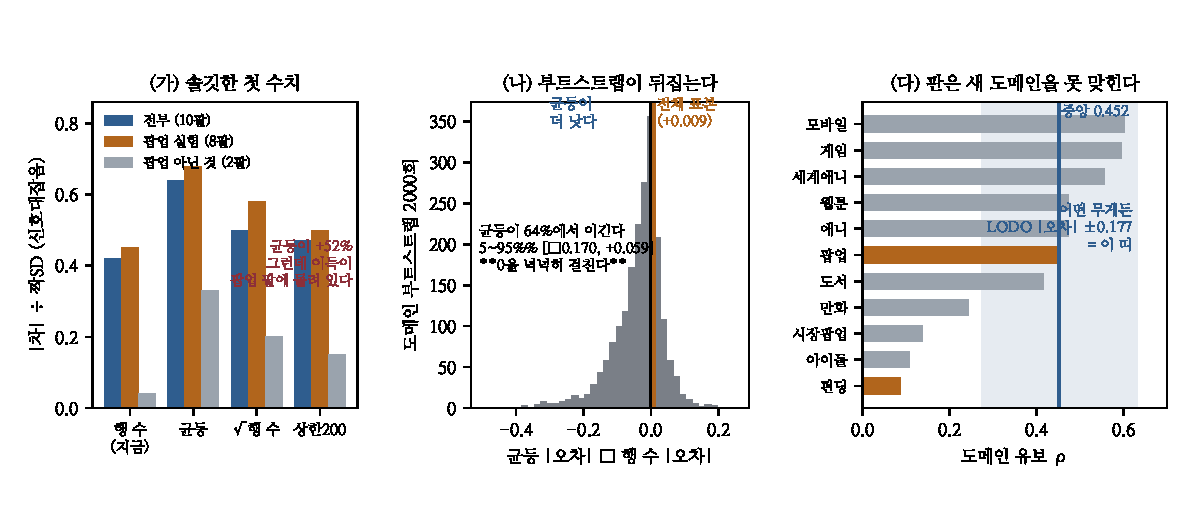
\includegraphics[width=\linewidth]{figs/fig380.pdf}
\caption{\textbf{(가)} 저장된 관문 열 팔을 규칙 넷으로 다시 판정한 신호대잡음.
균등이 제일 높지만 이득이 팝업 팔에 몰려 있다. \textbf{(나)} LODO
$|$오차$|$의 균등$-$행 수 차이를 도메인 부트스트랩 2,000회로 본 것 ---
전체 표본(주황)은 행 수 편인데 분포는 0을 넉넉히 걸치고 균등이 64\%에서
이긴다. \textbf{(다)} 도메인별 유보 $\rho$ 와 LODO $|$오차$|$ $\pm0.177$
띠. 띠가 사실상 전체를 덮는다.}
\label{fig:main}
\end{figure}

\section{첫 수치와 그것이 무너진 자리}

\begin{center}
\begin{tabular}{lrrrr}
\hline
규칙 & 판 & 짝 SD 중앙 & $|$차$|\div$SD & 팝업 몫 \\
\hline
행 수 (지금) & 0.4057 & 0.0034 & 0.42 & 1.9\% \\
균등 & 0.3767 & 0.0074 & \textbf{0.64} & 9.1\% \\
$\sqrt{\text{행 수}}$ & 0.3956 & 0.0045 & 0.50 & 4.4\% \\
상한 200 & 0.4001 & 0.0043 & 0.47 & 3.6\% \\
\hline
\end{tabular}
\end{center}

균등은 짝 SD가 2.2배로 커지지만 차이가 더 빨리 커져 신호대잡음이 좋아진다.
그리고 저장된 관문 열 팔에서 \textbf{방향이 바뀌는 팔이 없다} --- 바뀌는
것은 ``배포가 정한다''가 ``판이 정한다''로 옮겨 가는 것뿐이고, 노트 378이
배포 떠넘기기가 동전이 들어오는 자리라고 밝힌 참이라 그것도 이득으로
보였다.

\textbf{첫 번째 균열 --- 이득이 팝업 팔에 있다.} 균등은 팝업 몫을 4.8배로
올린다. 저장된 열 팔 중 여덟이 팝업 자료를 건드린 실험이니, 팝업이 움직인
실험에서 균등이 예민해지는 것은 발견이 아니라 산수다. 팝업 아닌 두 팔에서는
하나가 $0.05 \to 0.65$ 로 크게 좋아지고 하나는 $0.03 \to 0.01$ 로 그대로다
--- 그런데 뒤엣것은 노트 378이 36뽑기로 ``구별할 수 없음''을 확인한
진짜 영이라 \emph{좋아지면 안 되는} 팔이다. 즉 팝업 밖 증거는 사실상
한 팔이다.

\textbf{두 번째 균열 --- 추정 대상 시험이 안 갈린다.} 무게 규칙을 관문
예민도로 고르는 것은 순환이다. 규칙이 다른 것은 \emph{무엇을 추정하느냐}이니
그것으로 물어야 한다: 도메인 하나를 빼고 나머지 열로 그 도메인의 $\rho$ 를
맞히면 어느 규칙이 잘 맞히나.

\begin{center}
\begin{tabular}{lrrrr}
\hline
 & 행 수 & 균등 & $\sqrt{n}$ & 상한 200 \\
\hline
LODO $|$오차$|$ 평균 & \textbf{0.1772} & 0.1862 & 0.1804 & 0.1790 \\
도메인 부트스트랩에서 이긴 비율 & 28\% & \textbf{64\%} & 2\% & 6\% \\
\hline
\end{tabular}
\end{center}

\textbf{전체 표본과 부트스트랩이 서로 반대다.} 차이의 5\,--\,95\%가
$[-0.170,\ +0.059]$ 라 0을 넉넉히 걸친다. 도메인이 열하나뿐이라 어느
극단(펀딩 $+0.087$ · 모바일 $+0.602$)이 표본에 드느냐가 순위를 정한다.

\section{그래서 안 바꾼다}

노트 378이 만든 조항 ③은 ``결판이 안 나면 유지한다 --- 챔피언이 동점에서
이긴다''이다. 여기에 그대로 걸린다. \textbf{규칙을 고치려고 만든 조항이
규칙 자체에 처음 적용됐다.}

무게 규칙은 그대로 두되 노트 379가 드러낸 것은 대장에 남긴다:

\begin{enumerate}
\item 어떤 자료 결정이 한 도메인의 무게를 \textbf{두 배 넘게} 바꾸면,
판 변화를 \emph{수치가 옳아진 몫}과 \emph{무게가 바뀐 몫}으로 갈라
보고한다(노트 379의 표 모양).
\item 판과 함께 \textbf{도메인 중앙값}도 적는다. 지금은 판 0.4057 · 도메인
중앙 0.4522 · 도메인 평균 0.3767 이다. 셋이 벌어지면 무게가 일하고 있다는
뜻이다.
\end{enumerate}

\section{진짜 수확 --- 판은 새 도메인을 못 맞힌다}

네 규칙 모두 LODO $|$오차$|$가 $0.177 \sim 0.186$ 이다. 그런데 도메인
$\rho$ 자체가 중앙 $0.4522$ 둘레로 평균절대편차 $0.155$ · SD $0.197$ 로
퍼져 있다. \textbf{즉 판으로 새 도메인을 맞히는 것이 중앙값을 부르는 것과
거의 같다.}

노트 352가 도메인 쌍 45개 중 30개를 구별 못 한다고 적고 ``수준은 못
잰다''를 남겼는데, 이것은 그 문장의 도메인판이다 --- \textbf{판은 우리가
가진 열한 도메인을 요약하는 수이지 열두 번째를 예언하는 수가 아니다.}
관문에서 두 팔을 견주는 데는 그대로 쓸 수 있다(짝지어 재니 도메인 수준이
상쇄된다). 다만 ``판 0.41 이니 새 도메인에서도 0.41''은 근거가 없다.

\section{남은 것}

\begin{center}
\begin{tabular}{lll}
\hline
항목 & 왜 값이 큰가 & 어떻게 \\
\hline
도메인 열두 번째 & 판이 예언하는지 유일한 직접 시험 & 새 도메인 하나를 통째로 모아 예언과 대조 \\
균일 2,051건 학습 & 학습도 상위 19\% 다 & 채점 집합 고정, 학습만 넓혀 관문 \\
다른 아홉 바닥 검사 & 펀딩만 고치면 판이 더 어긋난다 & 노트 375 분류대로 \\
팝업 실측 41행 & 배포가 65행이다 & 수집 \\
\hline
\end{tabular}
\end{center}

\end{document}
